\chapter{Ap\'endice}
\section{Appendix 1: Transformaci\'on de Coordenadas}
\label{App1}

%[Montenbruck, Vallado Revisitin, Vallado Coorde Sys, tabla de Boado]

Para la comparaci\'on de las posiciones en coordenadas cartesianas, es necesario llevar ambos vectores a un mismo sistema de referencia.
La figura (ref) muestra un resumen de los distintos sistemas y las consideraciones de cada uno. 

\begin{figure}[!h]
  \centering
  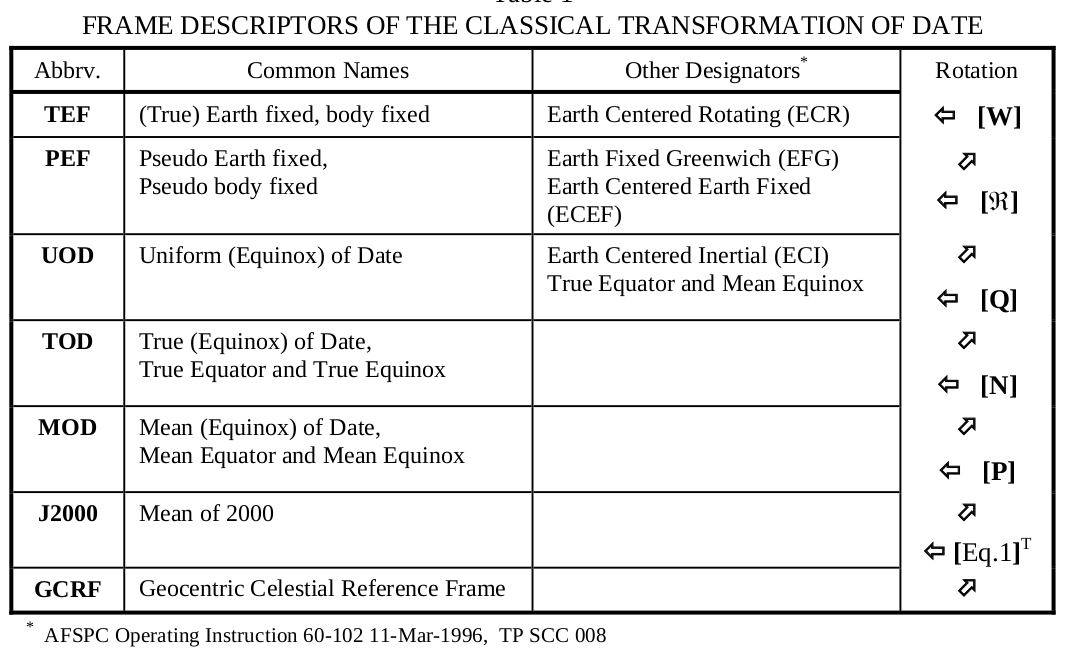
\includegraphics[width=0.7\textwidth]{imagenes/sistReferencias}
\end{figure}

En nuestro caso en particular, los datos que provee CODS se publican en el sistema TOD: True of Date (Verdadero de la \'epoca), mientras que los vectores de estado que genera el propagador SGP4 est\'an calculados en el sistema TEME: True Equator Mean Equinox (Ecuador Verdadero y Equinoccio Medio), tambi\'en denominado UOD (Uniform Equinox of Date).

Para la transformaci\'on de los datos de salida del SGP4 en el sistema TEME, al sistema TOD utilizamos la ecuaci\'on de los equinoccios, $EQ_{equinox}$, que nos permite transformar el equinoccio medio en el equinoccio verdadero.\\
Dado el vector de estado en el sistema TEME, $r_{_{TEME}}$, lo multiplicamos por la matriz de transformaci\'on en el eje z $Rot_{3}(EQ_{equinox})$ y obtenemos el vector de estado en el sistema TOD, $r_{_{TOD}}$.

\begin{equation}
 r_{_{TOD}} = [Q] r_{_{TEME}}
\end{equation}


 \[ Q =
\left( \begin{array}{ccc}
 cos(-EQ_{eqe}) & sin(-EQ_{eqe}) &  0 \\ 
 -sin(-EQ_{eqe}) & cos(-EQ_{eqe}) &  0 \\
 0 & 0 & 1
\end{array} \right) \] 


La ecuaci\'on de los equinoccios utiliza el modelo de nutaci\'on IAU-80 que considera los par\'ametros de nutaci\'on y los 106 coeficientes de Delaunay para el c\'alculo de la longitud $\Delta \Psi$ y la oblicuidad $\Delta \epsilon$.

\begin{equation}
 EQ_{eqe}=\Delta \Psi cos({\epsilon}) + 0.00264 \textquotedbl sin(\Omega_{(}) + 0.000063 \textquotedbl sin (2 \Omega_{(})
\end{equation}

Donde:

\begin{align*}
 \epsilon &= {\bar{\epsilon}} + \Delta \epsilon\\
 \Delta \Psi &= \sum_{i=1}^{106}  (A_{p} + A_{pl} tt) sin(a_{p_{i}})\\
 \Delta \epsilon &= \sum_{i=1}^{106}  (A_{e} + A_{el} tt) cos(a_{p_{i}})
\end{align*}

\begin{align*}
tt &=(jd-2451544.5)/36525.0 \\
 {\bar{\epsilon}} &= 84381.448 \textquotedbl - 46.8150 \textquotedbl tt - 0.00059 \textquotedbl tt^{2} + 0.001813 tt^{3}\\
 a_{p_{i}} &= a_{n1}M_{(}+a_{n2}M_{o}+a_{n3}\mu_{(}+a_{n4}D_{o}+a_{n5}\Omega_{(}
\end{align*}

Los coeficientes: $A_{p}$,$A_{pl}$,$A_{e}$,$A_{el}$,$a_{n_{i}}$ se extraen de la tabla de coeficientes de nutaci\'on de Seidelman, del libro de  \citep{montenbruck2012satellite}.

Y el resto de los par\'ametros se calcula seg\'un las expresiones:\\

\begin{align*}
    M_{(} &  = 134.96340251+1717915923.2178 tt+31.8792 tt^{2}+0.051 tt^{3}\\
    M_{o} & = 357.52910918+129596581.0481 tt-0.5532 tt^{2}-0.000136 tt^{3}\\
    \mu_{(} &= 93.27209062+1739527262.8478 tt-12.7512 tt^{2}-0.00103 tt^{3}\\
    D_{o} & = 297.85019547+1602961601.2090 tt-6.3706 tt^{2}+0.06593 tt^{3}\\
    \Omega_{(} & = 125.04455501-6962890.2665 tt+7.4722 tt^{2}+0.007702tt^{3}
\end{align*}

% \begin{figure}[!h]
%   \centering
%   \includegraphics[width=\textwidth]{imagenes/tablanutacion}
%   \caption{Teor\'ia de Nutaci\'on - \ac{IAU} 1980 - Tabla extra\'ida del libro de \citep{montenbruck2012satellite}}
%   \label{fig:tablaseidelman}
% \end{figure}

\newpage
%%%%%%%%%%%%%%%%%%%%%%%%%%%%%%%%
\section{Appendix 2: El archivo CDM}
\label{App2}

\lstset{language=XML,basicstyle=\small}
\begin{lstlisting}
<?xml version="1.0" encoding="UTF-8"?>
<cdm xmlns:xsi="http://www.w3.org/2001/XMLSchema-instance"
xsi:noNamespaceSchemaLocation="http://sanaregistry.org/r/ndmxml/ndmxml-1.0-master.xsd"
id="CCSDS_CDM_VERS" version="1.0">
<header>
<COMMENT>Sample CDM - XML version</COMMENT>
<CREATION_DATE>2010-03-12T22:31:12.000</CREATION_DATE>
<ORIGINATOR>JSPOC</ORIGINATOR>
<MESSAGE_FOR>SATELLITE A</MESSAGE_FOR>
<MESSAGE_ID>20111371985</MESSAGE_ID>
</header>
<body>
<relativeMetadataData>
  <COMMENT>Relative Metadata/Data</COMMENT>
  <TCA>2010-03-13T22:37:52.618</TCA>
  <MISS_DISTANCE units="m">715</MISS_DISTANCE>
  <RELATIVE_SPEED units="m/s">14762</RELATIVE_SPEED>
  <relativeStateVector>
    <RELATIVE_POSITION_R units="m">27.4</RELATIVE_POSITION_R>
    <RELATIVE_POSITION_T units="m">-70.2</RELATIVE_POSITION_T>
    <RELATIVE_POSITION_N units="m">711.8</RELATIVE_POSITION_N>
    <RELATIVE_VELOCITY_R units="m/s">-7.2</RELATIVE_VELOCITY_R>
    <RELATIVE_VELOCITY_T units="m/s">-14692.0</RELATIVE_VELOCITY_T>
    <RELATIVE_VELOCITY_N units="m/s">-1437.2</RELATIVE_VELOCITY_N>
  </relativeStateVector>
  <START_SCREEN_PERIOD>2010-03-12T18:29:32.212</START_SCREEN_PERIOD>
  <STOP_SCREEN_PERIOD>2010-03-15T18:29:32.212</STOP_SCREEN_PERIOD>
  <SCREEN_VOLUME_FRAME>RTN</SCREEN_VOLUME_FRAME>
  <SCREEN_VOLUME_SHAPE>ELLIPSOID</SCREEN_VOLUME_SHAPE>
  <SCREEN_VOLUME_X units="m">200</SCREEN_VOLUME_X>
  <SCREEN_VOLUME_Y units="m">1000</SCREEN_VOLUME_Y>
  <SCREEN_VOLUME_Z units="m">1000</SCREEN_VOLUME_Z>
  <SCREEN_ENTRY_TIME>2010-03-13T20:25:43.222</SCREEN_ENTRY_TIME>
  <SCREEN_EXIT_TIME>2010-03-13T23:44:29.324</SCREEN_EXIT_TIME>
  <COLLISION_PROBABILITY>4.835E-05</COLLISION_PROBABILITY>
  <COLLISION_PROBABILITY_METHOD>FOSTER-1992</COLLISION_PROBABILITY_METHOD>
</relativeMetadataData>
<segment>
  <metadata>
    <COMMENT>Object1 Metadata</COMMENT>
    <OBJECT>OBJECT1</OBJECT>
    <OBJECT_DESIGNATOR>12345</OBJECT_DESIGNATOR>
    <CATALOG_NAME>SATCAT</CATALOG_NAME>
    <OBJECT_NAME>SATELLITE A</OBJECT_NAME>
    <INTERNATIONAL_DESIGNATOR>1997-030E</INTERNATIONAL_DESIGNATOR>
    <OBJECT_TYPE>PAYLOAD</OBJECT_TYPE>
    <OPERATOR_CONTACT_POSITION>OSA</OPERATOR_CONTACT_POSITION>
    <OPERATOR_ORGANIZATION>EUMETSAT</OPERATOR_ORGANIZATION>
    <OPERATOR_PHONE>+49615130312</OPERATOR_PHONE>
    <OPERATOR_EMAIL>JOHN.DOE@SOMEWHERE>NET</OPERATOR_EMAIL>
    <EPHEMERIS_NAME>EPHEMERIS SATELLITE A</EPHEMERIS_NAME>
    <COVARIANCE_METHOD>CALCULATED</COVARIANCE_METHOD>
    <MANEUVERABLE>YES</MANEUVERABLE>
    <REF_FRAME>EME2000</REF_FRAME>
    <GRAVITY_MODEL>EGM-96: 36D 36O</GRAVITY_MODEL>
    <ATMOSPHERIC_MODEL>JACCHIA 70 DCA</ATMOSPHERIC_MODEL>
    <N_BODY_PERTURBATIONS>MOON,SUN</N_BODY_PERTURBATIONS>
    <SOLAR_RAD_PRESSURE>NO</SOLAR_RAD_PRESSURE>
    <EARTH_TIDES>NO</EARTH_TIDES>
    <INTRACK_THRUST>NO</INTRACK_THRUST>
  </metadata>
  <data>
    <COMMENT>Object1 Data</COMMENT>
    <odParameters>
    <COMMENT>Object1 OD Parameters</COMMENT>
    <TIME_LASTOB_START>2010-03-12T02:14:12.746</TIME_LASTOB_START>
    <TIME_LASTOB_END>2010-03-12T02:14:12.746</TIME_LASTOB_END>
    <RECOMMENDED_OD_SPAN units="d">7.88</RECOMMENDED_OD_SPAN>
    <ACTUAL_OD_SPAN units="d">5.50</ACTUAL_OD_SPAN>
    <OBS_AVAILABLE>592</OBS_AVAILABLE>
    <OBS_USED>59</OBS_USED>
    <TRACKS_AVAILABLE>123</TRACKS_AVAILABLE>
    <TRACKS_USED>119</TRACKS_USED>
    <RESIDUALS_ACCEPTED units="%" >97.8</RESIDUALS_ACCEPTED>
    <WEIGHTED_RMS>0.864</WEIGHTED_RMS>
    </odParameters>
    <additionalParameters>
    <COMMENT>Object 1 Additional Parameters</COMMENT>
    <AREA_PC units="m**2">5.2</AREA_PC>
    <MASS units="kg">2516</MASS>
    <CD_AREA_OVER_MASS units="m**2/kg">0.045663</CD_AREA_OVER_MASS>
    <CR_AREA_OVER_MASS units="m**2/kg">0.000000</CR_AREA_OVER_MASS>
    <THRUST_ACCELERATION units="m/s**2">0.0</THRUST_ACCELERATION>
    <SEDR units="W/kg">4.54570E-05</SEDR>
    </additionalParameters>
    <stateVector>
      <COMMENT>Object1 State Vector</COMMENT>
      <X units="km">2570.097065</X>
      <Y units="km">2244.654904</Y>
      <Z units="km">6281.497978</Z>
      <X_DOT units="km/s">4.418769571</X_DOT>
      <Y_DOT units="km/s">4.833547743</Y_DOT>
      <Z_DOT units="km/s">-3.526774282</Z_DOT>
    </stateVector>
    <covarianceMatrix>
      <COMMENT>Object1 Covariance in the RTN Coordinate Frame </COMMENT>
      <CR_R units="m**2">4.142E+01</CR_R>
      <CT_R units="m**2">-8.579E+00</CT_R>
      <CT_T units="m**2">2.533E+03</CT_T>
      <CN_R units="m**2">-2.313E+01</CN_R>
      <CN_T units="m**2">1.336E+01</CN_T>
      <CN_N units="m**2">7.098E+01</CN_N>
      <CRDOT_R units="m**2/s">2.520E-03</CRDOT_R>
      <CRDOT_T units="m**2/s">-5.476E+00</CRDOT_T>
      <CRDOT_N units="m**2/s">8.626E-04</CRDOT_N>
      <CRDOT_RDOT units="m**2/s**2">5.744E-03</CRDOT_RDOT>
      <CTDOT_R units="m**2/s">-1.006E-02</CTDOT_R>
      <CTDOT_T units="m**2/s">4.041E-03</CTDOT_T>
      <CTDOT_N units="m**2/s">-1.359E-03</CTDOT_N>
      <CTDOT_RDOT units="m**2/s**2">-1.502E-05</CTDOT_RDOT>
      <CTDOT_TDOT units="m**2/s**2">1.049E-05</CTDOT_TDOT>
      <CNDOT_R units="m**2/s">1.053E-03</CNDOT_R>
      <CNDOT_T units="m**2/s">-3.412E-03</CNDOT_T>
      <CNDOT_N units="m**2/s">1.213E-02</CNDOT_N>
      <CNDOT_RDOT units="m**2/s**2">-3.004E-06</CNDOT_RDOT>
      <CNDOT_TDOT units="m**2/s**2">-1.091E-06</CNDOT_TDOT>
      <CNDOT_NDOT units="m**2/s**2">5.529E-05</CNDOT_NDOT>
    </covarianceMatrix>
  </data>
</segment>
<segment>
  <metadata>
    <COMMENT>Object2 Metadata</COMMENT>
    <OBJECT>OBJECT2</OBJECT>
    <OBJECT_DESIGNATOR>30337</OBJECT_DESIGNATOR>
    <CATALOG_NAME>SATCAT</CATALOG_NAME>
    <OBJECT_NAME>FENGYUN 1C DEB</OBJECT_NAME>
    <INTERNATIONAL_DESIGNATOR>1999-025AA</INTERNATIONAL_DESIGNATOR>
    <OBJECT_TYPE>DEBRIS</OBJECT_TYPE>
    <EPHEMERIS_NAME>NONE</EPHEMERIS_NAME>
    <COVARIANCE_METHOD>CALCULATED</COVARIANCE_METHOD>
    <MANEUVERABLE>NO</MANEUVERABLE>
    <REF_FRAME>EME2000</REF_FRAME>
    <GRAVITY_MODEL>EGM-96: 36D 36O</GRAVITY_MODEL>
    <ATMOSPHERIC_MODEL>JACCHIA 70 DCA</ATMOSPHERIC_MODEL>
    <N_BODY_PERTURBATIONS>MOON,SUN</N_BODY_PERTURBATIONS>
    <SOLAR_RAD_PRESSURE>YES</SOLAR_RAD_PRESSURE>
    <EARTH_TIDES>NO</EARTH_TIDES>
    <INTRACK_THRUST>NO</INTRACK_THRUST>
  </metadata>
    <data>
    <COMMENT>Object2 Data</COMMENT>
    <odParameters>
    <COMMENT>Object2 OD Parameters</COMMENT>
    <TIME_LASTOB_START>2010-03-12T01:14:12.746</TIME_LASTOB_START>
    <TIME_LASTOB_END>2010-03-12T03:14:12.746</TIME_LASTOB_END>
    <RECOMMENDED_OD_SPAN units="d">2.63</RECOMMENDED_OD_SPAN>
    <ACTUAL_OD_SPAN units="d">2.63</ACTUAL_OD_SPAN>
    <OBS_AVAILABLE>59</OBS_AVAILABLE>
    <OBS_USED>58</OBS_USED>
    <TRACKS_AVAILABLE>15</TRACKS_AVAILABLE>
    <TRACKS_USED>15</TRACKS_USED>
    <RESIDUALS_ACCEPTED units="%" >97.8</RESIDUALS_ACCEPTED>
    <WEIGHTED_RMS>0.864</WEIGHTED_RMS>
    </odParameters>
    <additionalParameters>
    <COMMENT>Object2 Additional Parameters</COMMENT>
    <COMMENT>Apogee Altitude=768 km</COMMENT>
    <COMMENT>Perigee Altitude=414 km</COMMENT>
    <COMMENT>Inclination=98.8 deg</COMMENT>
    <AREA_PC units="m**2">0.9</AREA_PC>
    <CD_AREA_OVER_MASS units="m**2/kg">0.118668</CD_AREA_OVER_MASS>
    <CR_AREA_OVER_MASS units="m**2/kg">0.075204</CR_AREA_OVER_MASS>
    <THRUST_ACCELERATION units="m/s**2">0.0</THRUST_ACCELERATION>
    <SEDR units="W/kg">5.40900E-03</SEDR>
    </additionalParameters>
    <stateVector>
      <COMMENT>Object2 State Vector</COMMENT>
      <X units="km">2569.540800</X>
      <Y units="km">2245.093614</Y>
      <Z units="km">6281.599946</Z>
      <X_DOT units="km/s">-2.888612500</X_DOT>
      <Y_DOT units="km/s">-6.007247516</Y_DOT>
      <Z_DOT units="km/s">3.328770172</Z_DOT>
    </stateVector>
    <covarianceMatrix>
      <COMMENT>Object2 Covariance in the RTN Coordinate Frame</COMMENT>
      <CR_R units="m**2">1.337E+03</CR_R>
      <CT_R units="m**2">-4.806E+04</CT_R>
      <CT_T units="m**2">2.492E+06</CT_T>
      <CN_R units="m**2">-3.298E+01</CN_R>
      <CN_T units="m**2">-7.5888E+02</CN_T>
      <CN_N units="m**2">7.105E+01</CN_N>
      <CRDOT_R units="m**2/s">2.591E-03</CRDOT_R>
      <CRDOT_T units="m**2/s">-4.152E-02</CRDOT_T>
      <CRDOT_N units="m**2/s">-1.784E-06</CRDOT_N>
      <CRDOT_RDOT units="m**2/s**2">6.886E-05</CRDOT_RDOT>
      <CTDOT_R units="m**2/s">-1.016E-02</CTDOT_R>
      <CTDOT_T units="m**2/s">-1.506E-04</CTDOT_T>
      <CTDOT_N units="m**2/s">1.637E-03</CTDOT_N>
      <CTDOT_RDOT units="m**2/s**2">-2.987E-06</CTDOT_RDOT>
      <CTDOT_TDOT units="m**2/s**2">1.059E-05</CTDOT_TDOT>
      <CNDOT_R units="m**2/s">4.400E-03</CNDOT_R>
      <CNDOT_T units="m**2/s">8.482E-03</CNDOT_T>
      <CNDOT_N units="m**2/s">8.633E-05</CNDOT_N>
      <CNDOT_RDOT units="m**2/s**2">-1.903E-06</CNDOT_RDOT>
      <CNDOT_TDOT units="m**2/s**2">-4.594E-06</CNDOT_TDOT>
      <CNDOT_NDOT units="m**2/s**2">5.178E-05</CNDOT_NDOT>
    </covarianceMatrix>
  </data>
</segment>
</body>
</cdm>
\endinput
\end{lstlisting}

\newpage
%%%%%%%%%%%%%%%%%%%%%%%%%%%%%%%%
\section{Appendix 3: Gr\'aficos de las probabilidades de colisi\'on}
\label{App3}

Gr\'aficos con las PoC en funci\'on del radio de colisi\'on elegido. 
Resultados de las situaciones que analizan en su trabajo Xu y Xiong (\citep{xu2014method}).


\begin{figure}[!h]
  \centering
  \fbox{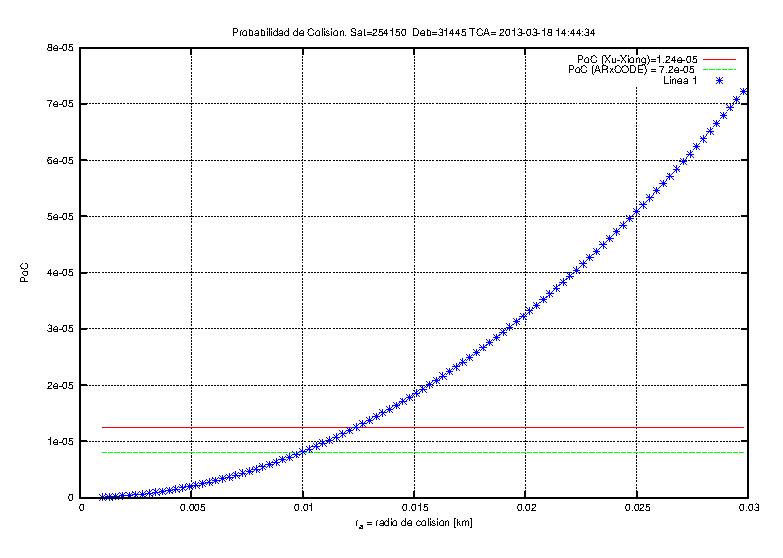
\includegraphics[width=0.6\textwidth]{imagenes/xuxiong1}}
  \caption{An\'alisis de la Probabilidad de Colisi\'on en funci\'on del radio de colisi\'on}
  \label{fig:pocvsraEsc4}
\end{figure}

\begin{figure}[!h]
  \centering
  \fbox{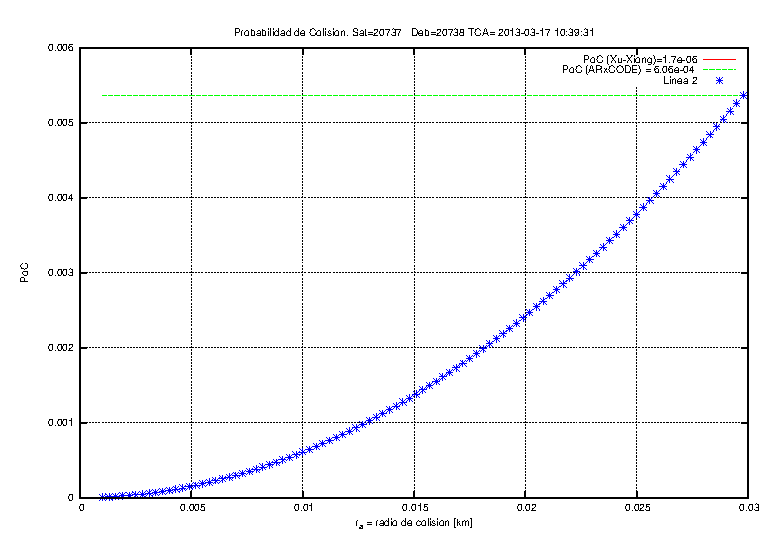
\includegraphics[width=0.6\textwidth]{imagenes/xuxiong2}}
  \caption{An\'alisis de la Probabilidad de Colisi\'on en funci\'on del radio de colisi\'on}
  \label{fig:pocvsraEsc5}
\end{figure}

\begin{figure}[!h]
  \centering
  \fbox{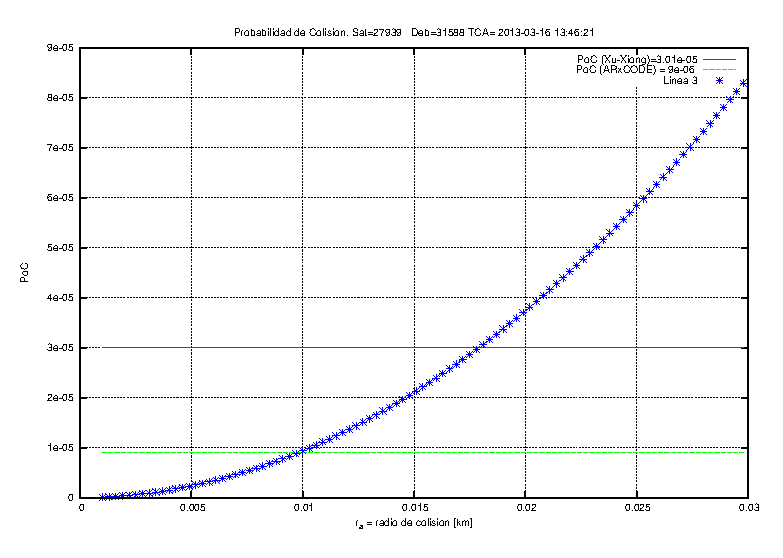
\includegraphics[width=0.6\textwidth]{imagenes/xuxiong3}}
  \caption{An\'alisis de la Probabilidad de Colisi\'on en funci\'on del radio de colisi\'on}
  \label{fig:pocvsraEsc4}
\end{figure}

\begin{figure}[!h]
  \centering
  \fbox{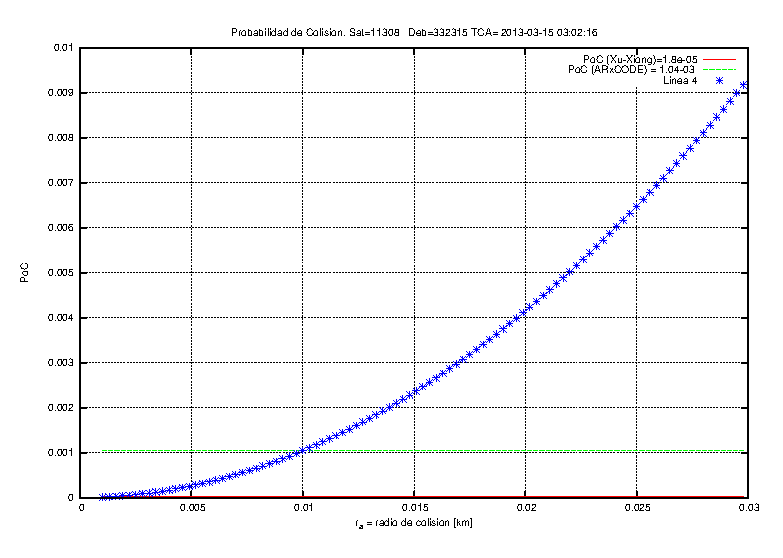
\includegraphics[width=0.6\textwidth]{imagenes/xuxiong4}}
  \caption{An\'alisis de la Probabilidad de Colisi\'on en funci\'on del radio de colisi\'on}
  \label{fig:pocvsraEsc5}
\end{figure}